\chapter{Tuning the models}

\section{Inertial circles in the dynamic model}

\begin{figure}
    \centering
        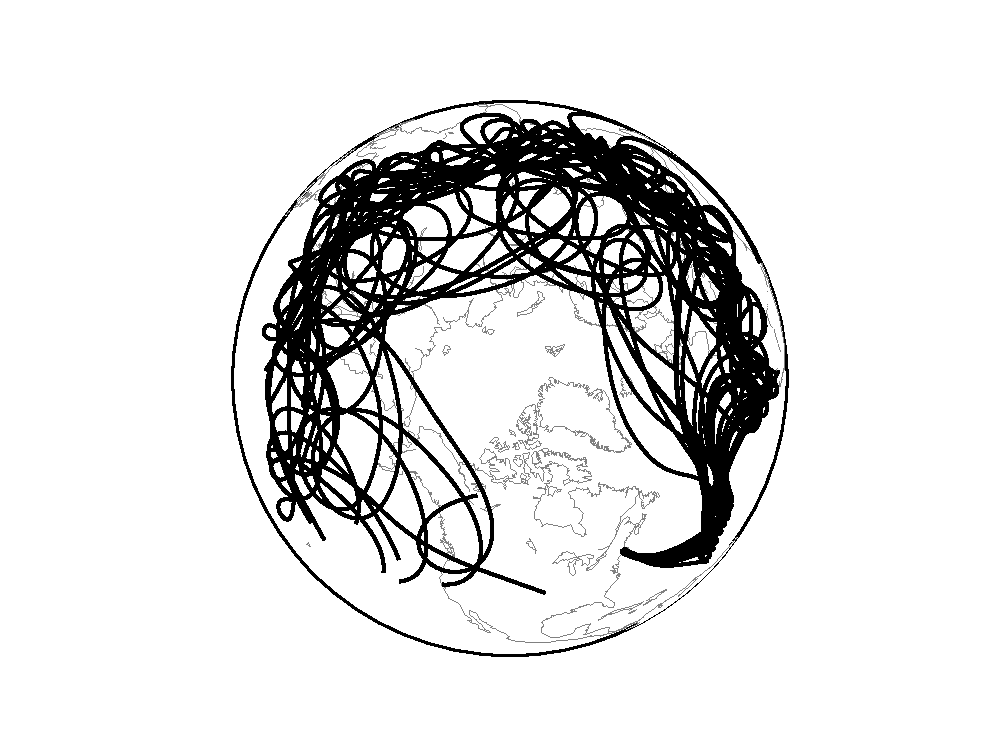
\includegraphics[trim=30 30 30 30, clip, width=0.49\textwidth]{force_180.eps}
        \includegraphics[trim=30 30 30 30, clip, width=0.49\textwidth]{friction_180.pdf}
    \caption{\textit{Left}: Twenty five trajectories calculated with the frictionless dynamic model. 
    Parcels were launched in an evenly-spaced 5x5 grid with its lower-left corner at 41, -72 and upper-right corner at 42, -71. 
    The large spirals are implausible for jet stream flow and reflect a problem with the model. 
    \textit{Right}: The same parcels with trajectories calculated by the dynamic model with friction.
    A few parcels still exhibit unrealistic spirals, but in general, trajectories are more plausible.}
    \label{fig:force_180}
\end{figure}

\section{Adding friction to the dynamic model}

[[[Inertial circles have been encountered before in dynamic models and there are different ways of dealing with them.]]] \cite{stohl_accuracy_1998}
One approach, used by Stohl and Seibert, is to take a weighted average of the wind speeds from the dynamic model and interpolated speeds from a kinematic model at each timestep.
Another approach is to change the frictionless assumption of the dynamical model.
[[[Why does the force of friction damp oscillations?]]]
Using the definition of geostrophic wind in Equations \ref{eq:u_g} and \ref{eq:v_g}, Equations \ref{eq:uvelocitygeo} and \ref{eq:vvelocitygeo} with an added friction term become

\begin{align}
    \frac{du}{dt} &= f (v - v_g) - r_f (u - u_g) \\
    \frac{dv}{dt} &= -f (u - u_g) - r_f (v - v_g).   
\end{align}

The friction parameter $r_f$ is analogous to the Coriolis parameter: it has units of second$^{-1}$ and is a measure of the force of friction.

\section{Choosing a timestep} \label{sec:timestep}
The threshold that HYSPLIT uses to calculate its dynamic timestep, Equation \ref{eq:threshold}, can also be expressed as the difference between a threshold velocity and trajectory velocity.

\begin{figure}
    \includegraphics[width=\textwidth]{speed_subplots_180_negative.pdf}
    \centering
    \caption{For a timestep of 3 minutes, trajectory speed is compared to threshold speed.
    Solid lines represent the threshold speed minus the trajectory speed for a timestep of 3 minutes. 
    The dashed line at a velocity of zero represents the speed threshold.
    Note in the upper-right hand plot that the zonal speeds for some trajectories surpass the threshold. }
    \label{fig:speed_subplots_180_negative}
\end{figure}

\begin{figure}
    \includegraphics[width=\textwidth]{speed_subplots_90_negative.pdf}
    \centering
    \caption{For a timestep of 1 minute and 30 seconds, trajectory speed is compared to threshold speed.
    For this choice of timestep, all parcel velocities are below the threshold.}
    \label{speed_subplots_90_negative}
\end{figure}

\section{Initializing velocity for the dynamic model}

\begin{figure}
    \centering
    \includegraphics[width=\textwidth]{speed_ratio.pdf}
    \caption{}
    \label{fig:speed_ratio}
\end{figure}
